Le diagramme de déploiement (Figure~\ref{fig:diagramme_deploiement}) illustre l’architecture du système, reliant les équipements médicaux, le backend et les interfaces utilisateur.

\begin{figure}[h]
    \centering
    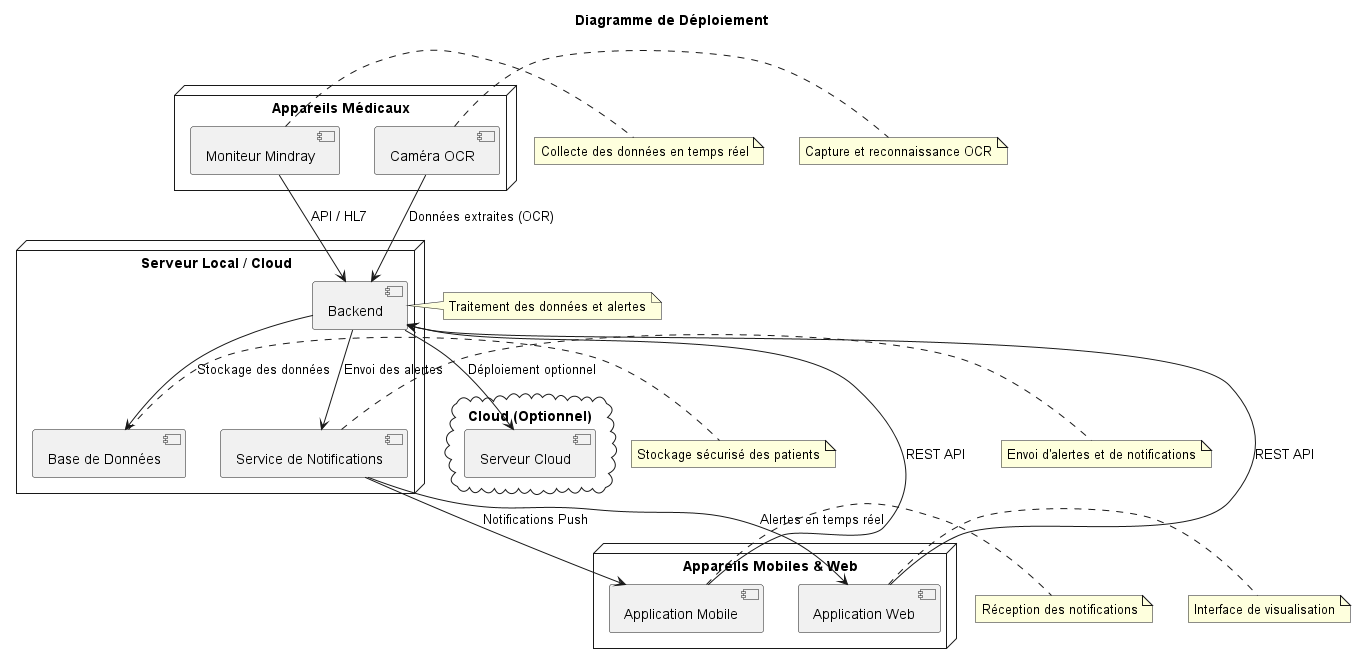
\includegraphics[width=1\textwidth]{chapter2/sections/diagrams/deployment_diagram.png}
    \caption{Diagramme de Déploiement du Système}
    \label{fig:diagramme_deploiement}
\end{figure}

\subsection{Composants et Déploiement}
\begin{itemize}
    \item \textbf{Serveur Local / Cloud} :
    \begin{itemize}
        \item \textbf{Backend} : Traitement des données et gestion des alertes.
        \item \textbf{Base de Données} : Stockage des patients et alertes.
        \item \textbf{Service de Notifications} : Envoi d’alertes (e-mails, push).
    \end{itemize}
    \item \textbf{Appareils Médicaux} :
    \begin{itemize}
        \item \textbf{Moniteur Mindray} : Envoie les données via API HL7.
        \item \textbf{Caméra OCR} : Capture et extrait les valeurs vitales.
    \end{itemize}
    \item \textbf{Applications Mobiles \& Web} :
    \begin{itemize}
        \item \textbf{Application Web / Mobile} : Consultation des données via REST API.
    \end{itemize}
\end{itemize}

\subsection{Flux de Communication}
\begin{enumerate}
    \item Collecte des données via HL7 ou OCR.
    \item Analyse et stockage par le backend.
    \item Détection des anomalies et envoi d’alertes.
    \item Consultation des alertes et données par le personnel médical.
\end{enumerate}

\subsection{Justification}
L’architecture garantit \textbf{modularité} (séparation des composants), \textbf{réactivité} (alertes en temps réel) et \textbf{interopérabilité} (compatibilité HL7 / OCR), avec une option de déploiement sur serveur local ou cloud.
